\documentclass[aspectratio=169]{beamer}
\usepackage[russian]{babel}
\usepackage[utf8]{inputenc}
\usepackage{verbatim}
\usepackage{graphicx}
\usepackage{pgfpages}
\usepackage{ulem}
\usepackage{float}
\usepackage{amsmath}

\setbeameroption{hide notes}

\setbeamercolor{title}{fg=white}
\setbeamercolor{author}{fg=white}
\setbeamercolor{normal text}{fg=black}
\setbeamercolor{frametitle}{fg=black}
\setbeamercolor{item}{fg=red}
\setbeamercolor{block title}{fg=red}
\setbeamercolor{section in toc}{fg=red}
\setbeamercolor{footline}{fg=white}
\setbeamercolor{title in head/foot}{fg=white,bg=black}

\setbeamertemplate{navigation symbols}{}
\setbeamertemplate{headline}{
    
\includegraphics[height=1mm, width=\paperwidth]{wg-headline.png}
}

\setbeamertemplate{footline}{
    \begin{beamercolorbox}[ht=1.2em]{title in head/foot}
        {\footnotesize \hspace{1em}\inserttitle, \insertshortauthor}
    \end{beamercolorbox}
}

\begin{document}

\title{World of Tanks: на пути к 1M CCU}
\author{Максим Мельников}
\date{}

{
\title{
    
\includegraphics[width=0.4\textwidth]{wg-logo.png}
    
\includegraphics[width=0.4\textwidth]{rit-logo-black.png}
    \\
    {\huge WORLD OF TANKS: НА ПУТИ К 1M CCU}
}
\author{МАКСИМ МЕЛЬНИКОВ}

\usebackgroundtemplate{
\includegraphics[width=\paperwidth]{wg-end.jpg}}
\begin{frame}[plain]{}
    \titlepage
    \note{
    Привет. Меня зовут Максим Мельников, я работаю в компании Wargaming.net,
и сегодня хотел бы рассказать вам о World of Tanks. На самом деле это первый 
технический доклад, от нашей компании, который рассказывает об архитектуре танков. 
Думаю вам будет интересно и полезно.
    }
\end{frame}
}

\usebackgroundtemplate{
\includegraphics[width=\paperwidth]{wg-bg.jpg}}
\logo{
    
\includegraphics[height=1.7cm]{wg-logo.png}
    \hspace{0.5em}
    
\includegraphics[height=1.7cm]{rit-logo-white.png}
    \hspace{0.5em}
}

\section{Вступление}
\begin{frame}{КТО Я}
    \begin{itemize}
        \item Wargaming.net
            \begin{itemize}
                \item \sout{Order of War}
                \item \sout{Order of War: Challenge}
                \item World of Tanks developer
            \end{itemize}
        \item Linux Mobile hobbyist
            \begin{itemize}
                \item \sout{Openmoko}
                \item systemd
                \item telepathy
                \item Gentoo
            \end{itemize}
    \end{itemize}
    \note{
    Сначала немного о себе. В компанию я пришёл 3.5 года назад, на проект Order of War.
Там я занимался выделением standalone "игрового сервера" и портированием его на Linux.

    После релиза Order of War: Challenge, перешёл на проект World of Tanks, 
где поработал над: поддержкой AMQP для игрового сервера; разработкой клановых войн; 
а также разработкой Wargaming.net ID (OpenID) сервиса.

    Кроме работы, меня интересует тема OpenSource и Linux-а на мобильных устройствах,
особенно всё, что касается systemd, telepathy и такого дистрибутива как Gentoo.
    }
\end{frame}

\begin{frame}{WORLD OF TANKS СЕГОДНЯ}
    \begin{itemize}
        \item 800k одновременно играющих в пике
        \item 8M сообщений в секунду
        \item 300 серверов для обслуживания игры
        \item 60M посещений игрового портала в месяц
        \item 5PB (петабайт) на установку и обновления игрового клиента в месяц
    \end{itemize}
    \note{
    На всякий случай: World of Tanks - это такая сессионная многопользовательская
ролевая игра про танки, где игроки, в командах по 15 человек, воют друг-против-друга
в стиле обычных шутеров, но на танках. С развитием танков, экипажа и т.д.

    Игра очень популярна, особенно на территории бывшего советского союза. Вот некоторая
статистика с этого региона:
более 800 тыс одновременно играющих в пике;
во время игры рассылается более 8 млн сообщений с игрового сервера в игровые клиенты в секунду;
обслуживанием только игры (без web-обвязки) занимается более 300 очень мощных серверов;
на главном web-портале игры - более 60 млн посещений в месяц;
и поскольку World of Tanks - клиентская игра,
очень много трафика уходит на установку и обновление игрового клиента - более 5 петабайт,
переформулирую, более 5 миллионов гигабайт в месяц.
    }
\end{frame}

\begin{frame}{СОДЕРЖАНИЕ}
    \tableofcontents
    \note{
    Вот некоторое содержание того, о чём мне хотелось бы вам рассказать. Начнём 
с общей архитектуры игрового сервера. Далее я расскажу про некоторые особенности трафика 
с сервера на клиент. Затем я постараюсь объяснить, зачем нам множество периферий: RU1, RU2, 
и т.д. и как это внутри работает. Потом переключимся на web - немаловажную обвязку вокруг
игры. И на сладкое, поделюсь особенностями раздачи обновление такому большому количеству
игроков.
    }
\end{frame}

\section{Фрагменты архитектуры}
\subsection{Игровой cервер}

\begin{frame}{АРХИТЕКТУРА WORLD OF TANKS}
    \begin{itemize}
        \item клиент игры --- тонкий клиент, плеер
        \item сервер --- расчёт игрового мира
        \item кластер --- сотни процессов работающих как единое целое (сервер)
        \item игровой мир --- пошаговый, шаги очень маленькие
    \end{itemize}
    \note{
    Саму архитектуру игры World of Tanks можно разделить на следующие компоненты:
Сервер - занимается всеми расчётами игры; клиент - является не более чем, весьма специфичным
плеером, который показывает данные приходящие с сервера, и передаёт управляющие команды на сервер.
При этом сам сервер - это тысячи процессов, работающих на сотнях серверов как единое целое.
Расчёты изменений игрового мира происходят пошагово, одно такое изменение мы называем тиком,
и сейчас у нас 10 тиков в секунду.
    }
\end{frame}

\begin{frame}{АРХИТЕКТУРА КЛАСТЕРА}
    \begin{columns}

    \begin{column}{0.33\textwidth}
    \begin{block}{Storage*}
        \begin{itemize}
            \item MySQL
            \item MySQL*
            \item RabbitMQ
        \end{itemize}
    \end{block}
    \end{column}

    \begin{column}{0.33\textwidth}
    \begin{block}{Nodes}
        \begin{itemize}
            \item BaseApp
            \item CellApp
            \item LoginApp
        \end{itemize}
    \end{block}
    \end{column}

    \begin{column}{0.33\textwidth}
    \begin{block}{Managers}
        \begin{itemize}
            \item BaseAppMgr
            \item CellAppMgr
            \item DbMgr
        \end{itemize}
    \end{block}
    \end{column}

    \end{columns}
    \vspace*{1cm}

    \note{
    Игровой сервер состоит нескольких компонентов:
BaseApp - тут происходит "игра в ангар";
BaseAppMgr - Управляющий сервис для BaseApp-ов, занимается балансировкой и хранит глобальные данные;
на CellApp живут "объекты" боевых арен;
CellAppMgr по выполняемым задачам аналогичен BaseAppMgr, только занимается он CellApp-ами;
LoginApp - cервис отвечающий за взаимодействие с клиентом во время входа в игру;
DbMgr - управляет работой базы данных, следит за всеми сущностями;
MySQL - база данных, которая хранит аккаунты пользователей;
RabbitMQ - не нужен для работы самого кластера, а только как средство RPC с Web-ом, но об этом потом.
    }
\end{frame}

\begin{frame}{АРХИТЕКТУРА КЛАСТЕРА II}
    \begin{columns}
        \begin{column}{0.4\textwidth}
        \begin{block}{BaseApp}
        \begin{itemize}
            \item Account
            \item ChatChannel
            \item Clan
            \item Admin
            \item SysMessenger
            \item Node
        \end{itemize}
        \end{block}
        \end{column}

        \begin{column}{0.4\textwidth}
        \begin{block}{CellApp}
        \begin{itemize}
            \item Arena
            \item Avatar
            \item Vehicle
            \item TeamBase
            \item AreaDestructibles
            \item Node
        \end{itemize}
        \end{block}
        \end{column}
    \end{columns}
    \vspace*{1cm}

    \note{
    Немного о том, чем занимаются BaseApp, и CellApp, за какие объекты отвечают и что делают.
С точки зрения ОС, это однопоточные процессы, по этому на одном физическом сервере их запущенно
несколько - по количеству ядер в системе. На каждом из их, живёт по одному специальному объекту
Node - который занимается низкоуровневыми задачами, необходимым для работы кластера.

    BaseApp - процесс, который занимается обслуживанием соединения с клиентами и обслуживанием
аккаунта игрока: покупки в магазине; чат; вход в бой и т.д. и т.п - в общем всё то, что делает
человек в ангаре. Так же на нём живут "сущности" клана, админа, чата и т.д.

    CellApp - это процесс, который занимается обслуживанием боёв. В одном бою участвуют 
множество различных обектов: арена, танк, аватар, база команды и специальные объекты которые
отвечают за разрушаемость сцены и т.д.
    }
\end{frame}

\begin{frame}{РАЗРАБОТКА СЕРВЕРА}
    \begin{enumerate}
        \item обычный Python
        \item GC выключен
        \item немного C++
        \item RPC - на базе сообщений
        \item UDP-based протокол с гарантией доставки
    \end{enumerate}
    \note{
    Для разработки сервера в основном используется Python. Для обеспечения работы в реальном
времени, GC выключен, ну и код пишется с учётом этого, чтобы сервер мог работать без рестарта
сервера. Самые узкие места, переписываются на C++, но их совсем немного. 
Логика игры пишется в обычном синхронном режиме, пока дело происходит в рамках одной
сущности. Если же необходимо взаимодействие с другими сущностями, они чаще всего живут на
других машинах, то обращение происходит асинхронно через внутренний механизм сообщений.
Внутри кластера, эти сообщения ходят между процессами по протоколу базирующимся на UDP,
с гарантией доставки.
    }
\end{frame}

\begin{frame}{ОТКАЗОУСТОЙЧИВОСТЬ}
    \begin{itemize}
        \item объекты только в памяти
        \item репликация объектов на случай отказа
    \end{itemize}
    \note{
    Поскольку все объекты живут только в памяти, проблема потери данных из-за падений встаёт
на первое место. Периодически состояние аккаунта сбрасывается в базу данных, однако оперативное
сбрасывание данных при таком онлайне не возможно. Возникает опасность отката данных аккаунта
на несколько минут, или даже часов. Для обеспечения отказоустойчивости все объекты периодически
бэкапируются, на соседние ноды. B случае её падения, BaseAppMgr выберет один из бэкапов, 
и сделает его активным.
    }
\end{frame}

\subsection{Сетевой трафик}

\begin{frame}{СЕТЕВОЙ ТРАФИК}
    \begin{enumerate}
    \item 8M уникальных UDP пакетов в секунду
    \item 16 Gbps на 800k пользователей
    \end{enumerate}
    \note{
    Огромное количество игроков в онлайне генерирует уйму сетевого трафика к игрокам.
Игровой мир движется маленькими шажками (тиками): 10/секунду. И после каждого шага, 
все подключённые пользователи получают синхронизирующие пакеты. Почти все пакеты 
обновления позиций танков, они могут теряться. Но есть и управляющие(RPC, статусы) 
команды, для которых реализована гарантия доставки.
    }
\end{frame}

\begin{frame}{НЕРАВНОМЕРНЫЙ ТРАФИК}
    \begin{itemize}
    \item 800k пакетов в 1ms
    \item 10k пакетов в следующие 99ms
    \end{itemize}
    \note{
    Главная проблема трафика - он очень неравномерный, в разрезе одной секунды.
Из-за пошаговости мира, и внутренней архитектуры движка пакеты игрокам в общем
случае рассылаются одновременно. Что вызывает огромную нагрузку на сетевое оборудование
в датацентрах, у провайдеров и т.д., в определённые миллисекунды, и фактически простой
в остальное время.

    Как мы с этим боремся? А никак. Настраиваем/покупаем оборудование, консультируем
провайдеров, устраиваем тестовые запуски и т.д. На самом деле, у нас есть механизм
включения рандомизации задержки в определённом малом промежутке времени, но с точки зрения
пользователя - это фактически увеличения задержки - по этому прибегаем только
в исключительных случаях, в основном при вводе новой периферии в игру, пока операторы и мы
настраиваем своё сетевое оборудование (вопрос нескольких дней).
    }
\end{frame}

\subsection{Метакластер}

\begin{frame}{ПРОБЛЕМЫ РОСТА}
    \begin{itemize}
    \item совсем не угадали размер аудитории на старте
    \item постоянный рост аудитории
    \item недоработки и нехватка оборудования
    \item постоянный аврал
    \item предел масштабирования кластера
    \end{itemize}
    \note{
    С самого релиза у нас постоянно возникали проблемы с ростом нагрузки, это были
не проблемы архитектуры, а различного рода недоработки и нехватка оборудования. Сколько
его не добавлялось, пользователей приходило всё больше. Достаточно долго разработчики и админы
жили в режиме постоянно аврала

    Со временем стало ясно, что у игрового движка есть некоторый предел масштабирования.
Где-то в роёне 250 тыс человек. Встал вопрос как жить дальше. При этом сразу поступило 
"ультимативное бизнес требование" - регион на шарды не делить.
    }
\end{frame}

\begin{frame}{ПЕРЕЕЗДЕЦ}
    \begin{itemize}
        \item много кластеров
        \item быстрое перемещение между кластерами
        \item выделенный кластер для хранения данных
    \end{itemize}
    \note{
    Для решения проблемы масштабирования решили вводить несколько кластеров, и дать игрокам
простой,понятный и быстрый механизм переключения между ими. Правда в таких условиях становится
сложно понять, где в данный момент данные, не потерялись ли посредине. И как в случае 
падений и отказов искать более последнюю копию, при этом желательно автоматически.

    Для этого решили выделить ещё один, отдельный кластер - центральный, который является
хранилищем данных, а остальные (периферии) сделать игровыми. Фича получила название - переездец.
    }
\end{frame}

\begin{frame}{АРХИТЕКТУРА МЕТАКЛАСТЕРА}
    \begin{columns}

    \begin{column}{0.5\textwidth}
    \begin{block}{Центр}
        \begin{itemize}
            \item постоянное хранилище
            \item аккаунты (proxy)
            \item взаимодействие с web-ом
        \end{itemize}
    \end{block}
    \end{column}
    
    \begin{column}{0.5\textwidth}
    \begin{block}{Периферия RU1, RU2, ...}
        \begin{itemize}
            \item временное хранилище
            \item аккаунты
            \item бои
        \end{itemize}
    \end{block}
    \end{column}

    \end{columns}
    \note{
    После разделения, разделились и обязанности и роли. Центральный сервер отвечает за взаимодействие
с web-ом, на нём же хранятся данные по всем аккаунтам, и подняты все аккаунты которые сейчас онлайн,
на любой из периферий. На перифериях происходят бои, покупка/продажа танков и т.д. При логине на периферию
приезжает аккаунт целиком, при выходе - commit-ится на центр. Так же, во время игры центр и периферия
могут обмениваться сообщениями о различных изменениях аккаунтов: начисления золота, приглашения в бои,
экспорт данных.
    }
\end{frame}

\begin{frame}{ПРEИМУЩЕСТВА МЕТАКЛАСТЕРА}
    \begin{enumerate}
        \item масштабируемость
        \item гео-распределённость
        \item отказоустойчивость
        \item независимость
    \end{enumerate}
    \note{
    Теперь проблема масштабируемый игрового сервера в принципе решена. Существует большой
запас по росту нагрузки центрального кластера, а трафик между кластерами совсем не большой.
Кроме того, были получены важные дополнительные преимущества, о которых раньше, честно говоря
не особо задумывались: появилась возможность разворачивать игровые сервера, по ближе к игрокам,
чтобы у их был меньший ping, и играть было комфортнее - в Мюнхене и Новосибирске; значительно
возросла отказоустойчивость всей системы - в случае проблем на одном из кластеров - это не
касается игроков на других кластерах, потеря связи с центром - тоже не проблема,
где-то до 30 минут - в этом случае единственное, что нельзя будет сделать - это залогиниться.
    Так же есть и "политические" преимущества, мы не зависим ни от конкретных датацентов,
ни от операторов трафика к датацентрам, у нас всегда есть возможность перенести кластер
в другое место, или развернуть дополнительный.
    }
\end{frame}

\subsection{Веб}

\begin{frame}{ВЕБ}
    \begin{columns}
        \begin{column}{0.4\textwidth}
        \begin{itemize}
            \item регистрация
            \item новости
            \item статьи и описания
            \item медиа контент
            \item платёжная форма
            \item обработка платежей
        \end{itemize}
        \end{column}

        \begin{column}{0.4\textwidth}
        \begin{itemize}
            \item раздача обновлений
            \item управление пользователями
            \item профиль игрока
            \item статистика
            \item рейтинги
            \item ...
        \end{itemize}
        \end{column}
    \end{columns}

    \note{
    Современная игра, не может обойтись без огромной web-обвязки: регистрация, новости, статьи, 
медиа-контент - тут всё понятно.

    Платежи - настолько большая и серьёзная тема, что её принято делить на 2 части - форма,
которая должна вызывать у пользователя желание платить и вообще очень сложная задача в плане UI и UX,
и некоторая платёжка - сервис который получает информацию от платёжных систем и агрегаторов - где
очень много вопросов по поддержке различных сервисов, конвертации валют, комиссий и т.д.

    Не стоит также забывать о задаче обновления самого игрового клиента.

    Реализация всего этого, уже годами отработана мировым сообществом на классических web-технологиях
и естественно у нас не было и мыслей об реализации всего этого на уровне игрового движка.
Не говоря уже о том, что всё это должно быть работоспособным в случае проблема на сервере.

    Весьма важный вопрос - некоторый публичный профиль, чтобы дать ссылку друзьям, и место где можно
сравнить кто круче, и/или вообще вынести в web часть игры.
    }
\end{frame}

\begin{frame}{ИНТЕГРАЦИЯ С ИГРОВЫМ СЕРВЕРОМ}
    \begin{itemize}
        \item AMQP --- протокол взаимодействия с игровым сервером
        \item XML-RPC обёртка над AMQP
        \item реплика данных игры в реляционном виде
    \end{itemize}
    \note{
    Web отдельно, игра отдельно - надо их как-то интегрировать. Взаимодействие с игровым сервером строится
по принципу чёрного ящика, для реализации API мы выбрали AMQP. Для упрощения разработки, 

    В web проектах достаточно часто и много необходимо обращаться в данным из игрового сервера, а сервер
хоть и хранит их в базе, но большая часть в очень неудобном виде - специальных блобах. Для упрощения, и 
    
    }
\end{frame}

\begin{frame}{СЕРВИСНАЯ АРХИТЕКТУРА}
    \begin{itemize}
        \item множество различных проектов
        \item протоколы взаимодействия: AMQP, HTTP, SQL, XML-RPC
    \end{itemize}
    \note{Отдельная задача - отдельный web проект}
\end{frame}

\begin{frame}{СТЭК ТЕХНОЛОГИЙ}
    \begin{columns}
        \begin{column}{0.4\textwidth}
            \begin{block}{LNAMPMR}
            \begin{itemize}
                \item Linux
                \item nginx
                \item Apache (mod\_wsgi)
                \item MySQL
                \item Python (Django)
                \item memcached
                \item RabbitMQ
            \end{itemize}
            \end{block}
        \end{column}

        \begin{column}{0.4\textwidth}
            \begin{block}{Другое}
            \begin{itemize}
                \item uwsgi
                \item Twisted
                \item Php
                \item Ruby
                \item PostgreSQL
                \item MongoDB
                \item Redis
            \end{itemize}
            \end{block}
        \end{column}
    \end{columns}
\end{frame}

\subsection{Обновление клиента}

\begin{frame}{ОБНОВЛЕНИЕ КЛИЕНТА}
    \begin{itemize}
        \item отдельный процесс который занимается обновлениями
        \item поддержка http и torrent протоколов
        \item 2M игроков
        \item размер обновления 1GB
        \item нет возможности раздавать обновление заранее
        \item короткая сессия участия игроков в раздаче
    \end{itemize}
    \note{
    Описание того, как много нужно раздать обновлений во время релиза.
Очень много желающих, раздача одновременно с релизом.
    }
\end{frame}

\begin{frame}{CБОР СТАТИСТИКИ}
    \begin{enumerate}
        \item Launcher
            \begin{itemize}
                \item файл
                \item размер
                \item время
                \item протокол
                \item источник
            \end{itemize}
        \item tracker
        \item CDN
    \end{enumerate}
    \note{Каждое скачивание - кто, что, как, откуда, сколько и с какой скоростью}
\end{frame}

\begin{frame}
    \frametitle{РЕШЕНИЕ}
    \begin{itemize}
        \item наши torrent сервера --- всегда в top-е
        \item web seed-ы
    \end{itemize}
    \hspace*{2cm}
    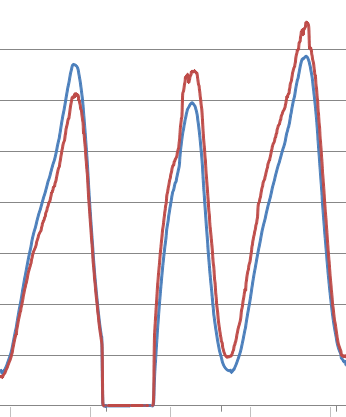
\includegraphics[height=0.5\textheight]{ccu.png}
    \note{Активное использование web seed-ов, патч на tracker}
\end{frame}

\section{Заключение}
{
\usebackgroundtemplate{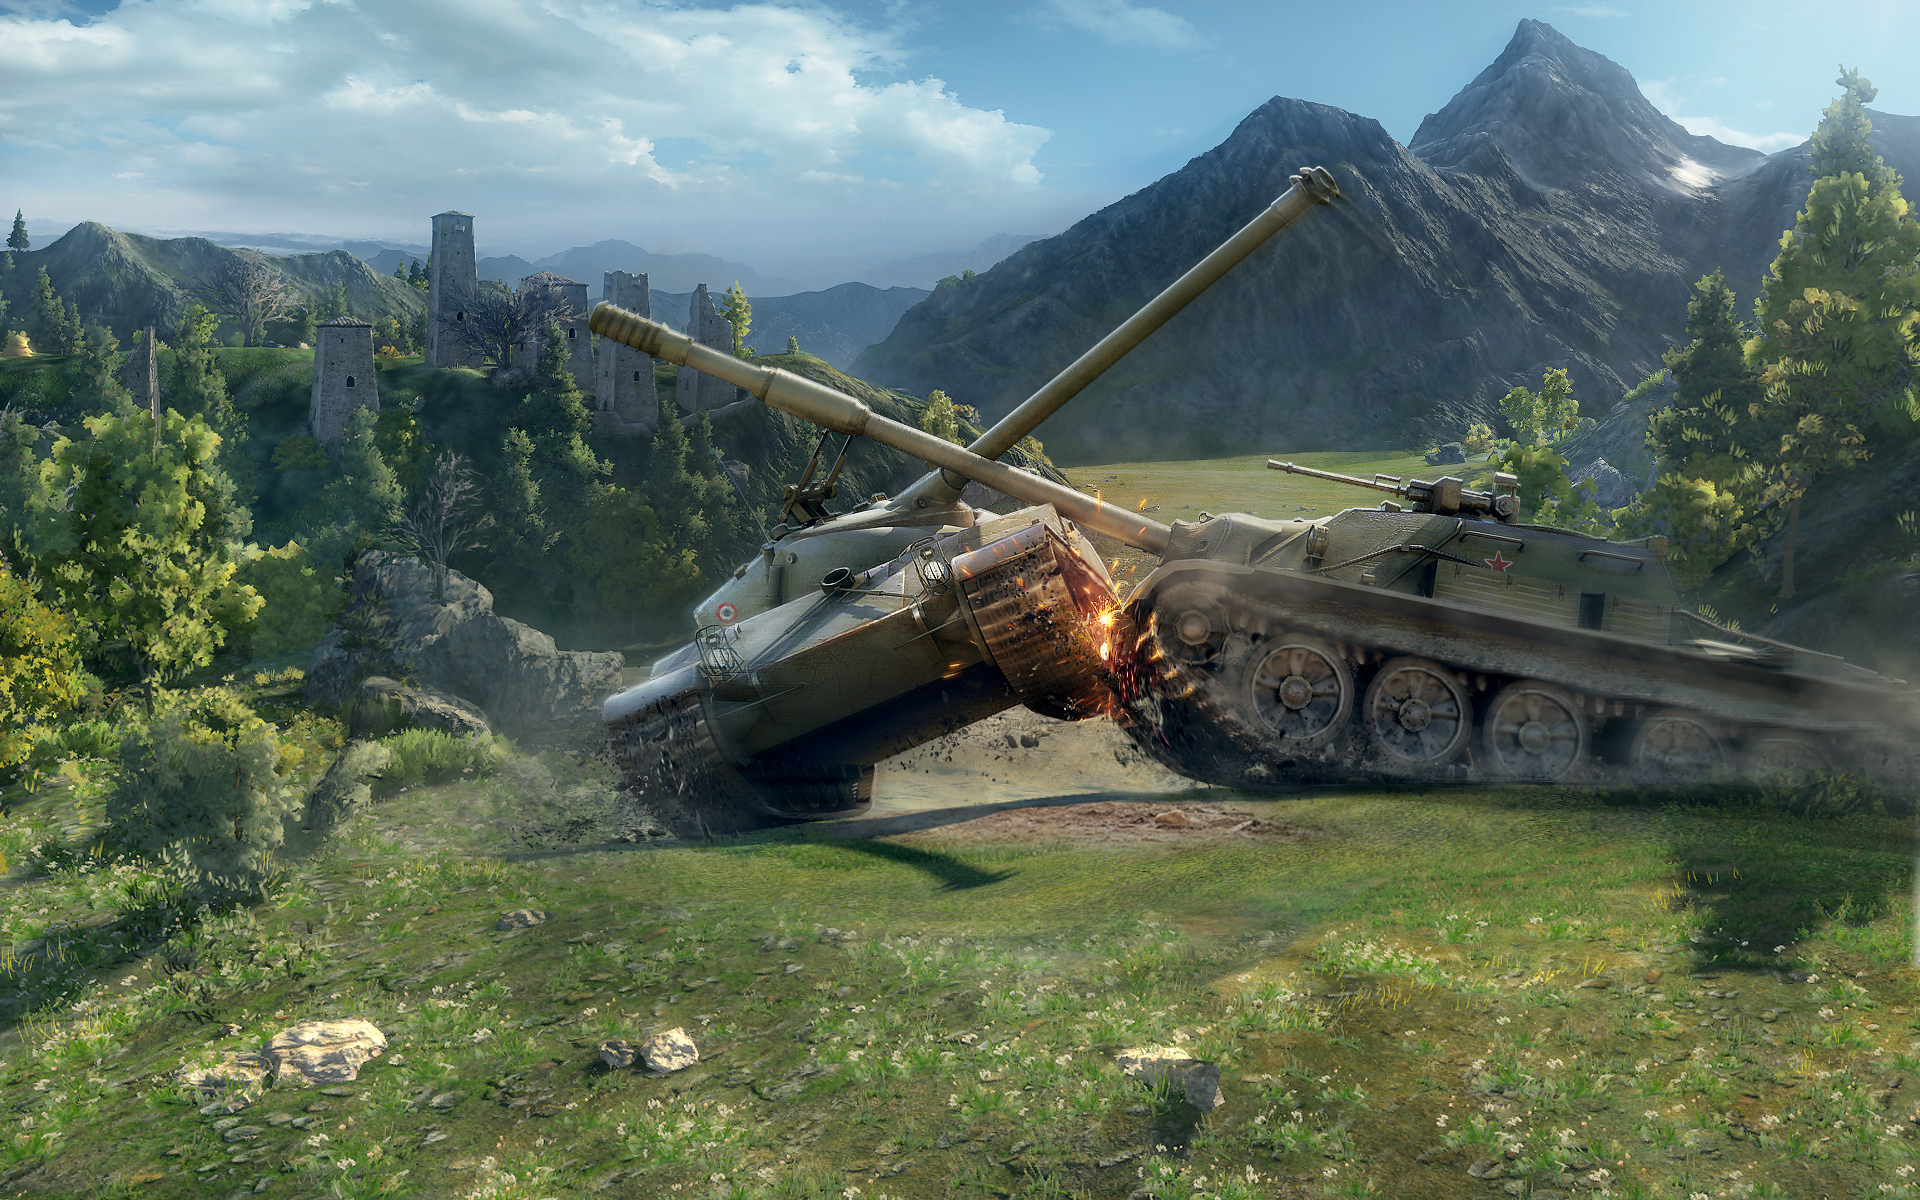
\includegraphics[width=\paperwidth]{wot.jpg}}
\begin{frame}[plain]{}
\note{Всё это и много другое, делается для того, чтобы игроки могли порубиться в танчики.}
\end{frame}
}

\begin{frame}{ИДЕИ}
    \begin{itemize}
        \item главное --- скорость и простота разработки
        \item не стоит боятся гетерогенной среды
        \item синхронный подход везде где можно
        \item асинхронный --- только там, где это необходимо
        \item AMQP --- отличный протокол для реализации RPC
        \item работа с объектами в памяти самая быстрая
    \end{itemize}
    \note{Главные идеи, которые можно было почерпнуть из доклада}
\end{frame}

{
\setbeamertemplate{footline}{}

\logo{
    
\includegraphics[height=1.7cm]{wg-logo.png}
    \hspace{0.2cm}
    
\includegraphics[height=1.7cm]{rit-logo-black.png}
    \hspace{0.2cm}
}

\setbeamercolor{frametitle}{fg=white}
\setbeamercolor{normal text}{fg=white}
\setbeamercolor{block title}{fg=white}
\setbeamercolor{block body}{fg=red}

\usebackgroundtemplate{
\includegraphics[height=\paperheight]{wg-end.jpg}}
\begin{frame}{СПАСИБО ЗА ВНИМАНИЕ. ВОПРОСЫ}
    \begin{block}{Максим Мельников}
    \par \url{mailto:m\_melnikau@wargaming.net}
    \par \url{https://plus.google.com/114669104565190507739/}
    \par \url{https://twitter.com/max\_posedon}
    \par \url{http://wargaming.com}
    \end{block}
\end{frame}
}

\begin{frame}{КОНФИГУРАЦИЯ ТИПИЧНОГО СЕРВЕРА}
    \begin{itemize}
        \item 2 cpu $*$ 8 core $*$ 2 threads
        \item 64 GB RAM
        \item 4 ethernet
    \end{itemize}
\end{frame}

\begin{frame}{ОСНОВНАЯ ИГРОВАЯ БАЗА}
    \begin{itemize}
        \item размер базы: 300 GB
        \item 384 GB RAM
        \item Percona 5.5 (разогрев кэша --- 1GBps)
        \item 40k select-ов, 1k insert-ов, 1k update-ов в секунду
        \item 24 HDD $*$ 600 GB $*$ 0.5 = 6 TB
    \end{itemize}
\end{frame}

\begin{frame}{ДОПОЛНИТЕЛЬНАЯ ИГРОВАЯ БАЗА}
    \begin{itemize}
        \item размер базы: 4 TB
        \item 64 GB RAM
        \item MySQL 5.5
        \item 100 GB, 350 млн записей (в день); 1k insert-ов в секунду
        \item 24 HDD $*$ 600 GB $*$ 0.5 $=$ 6 TB
        \item ext4
    \end{itemize}
\end{frame}

\end{document}
